\section{Results and Analysis}
\label{sec:results}



Table~\ref{tab:mainresults} presents the overall accuracy across all systems and LLMs. VersionRAG with DeepSeek-R1 70B achieves 90\% overall accuracy, significantly outperforming both Naive RAG (58\%) and GraphRAG (64\%). This 32 percentage point improvement over Naive RAG and 26 points over GraphRAG demonstrates the critical importance of version-aware retrieval. Notably, VersionRAG maintains its advantage across all model sizes, with even the smallest model (Llama 3 8B) achieving comparable performance to GraphRAG's best configuration.

\begin{table}[hb]
\centering
\small
\caption{Overall accuracy by query category. VersionRAG (our approach) consistently outperforms baselines across all configurations.}
\resizebox{\columnwidth}{!}{%
\begin{tabular}{llcccc}
\hline
LLM & Approach & Overall & Content & Version & Change \\
& & [\%] & Retrieval [\%] & Listing [\%] & Retrieval [\%] \\ \hline
\multirow{3}{*}{DeepSeek-R1 70B} 
& Naive RAG & 58.0 & 76.6 & 35.0 & 25.0\\
& GraphRAG & 64.0 & 70.0 & 80.0 & 30.0\\
& VersionRAG (ours) & \textbf{90.0} & \textbf{93.3} & \textbf{100.0} & \textbf{70.0}\\ \hline
\multirow{3}{*}{GPT-4o Mini} 
& Naive RAG & 53.0 & 70.0 & 20.0 & 35.0\\
& GraphRAG & 57.0 & 61.6 & 65.0 & 35.0\\
& VersionRAG (ours) & \textbf{79.0} & \textbf{80.0} & \textbf{90.0} & \textbf{65.0}\\ \hline
\multirow{3}{*}{Llama 3 8B} 
& Naive RAG & 47.0 & 61.6 & 25.0 & 25.0\\
& GraphRAG & 43.0 & 45.0 & 70.0 & 10.0\\
& VersionRAG (ours) & \textbf{55.0} & \textbf{61.6} & \textbf{70.0} & 20.0\\ \hline
\end{tabular}
}
\label{tab:mainresults}
\end{table}

\subsection{Performance by Query Type}

\paragraph{Content Retrieval.}
For standard content retrieval without version constraints, VersionRAG achieves 93.3\% accuracy with DeepSeek-R1 70B, slightly outperforming Naive RAG (76.6\%). The improvement stems from VersionRAG's metadata-enhanced retrieval, which filters out temporally irrelevant content even when version-specificity is not explicitly required. However, for version-specific content retrieval, the gap widens dramatically: VersionRAG achieves perfect 100\% accuracy while Naive RAG drops to 55\%. Figure~\ref{fig:contentretrievalversionspecificfailure} illustrates this failure mode—Naive RAG retrieves semantically similar content from multiple versions, creating ambiguity that prevents correct answers.

\begin{figure}[ht]
    \centering
    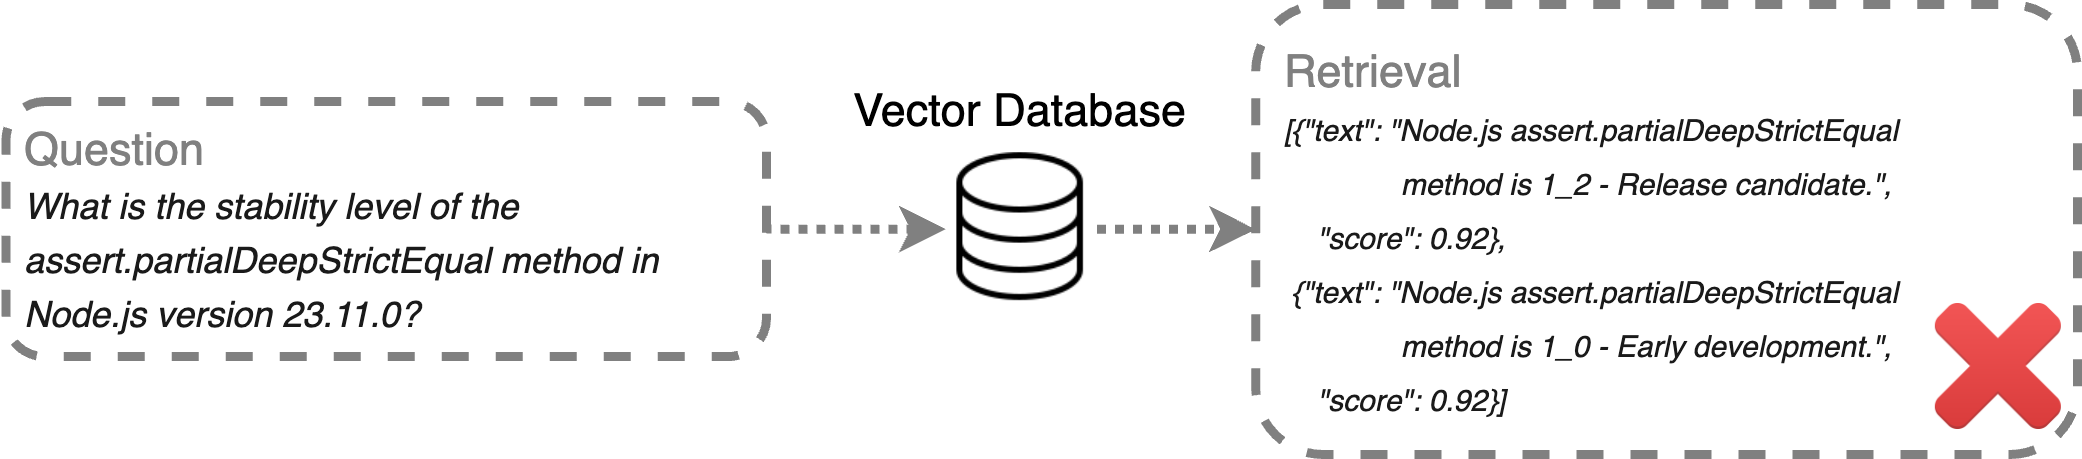
\includegraphics[width=1.0\columnwidth]{Figures/results_baseline_version_specific_retrieval.png}
    \caption{Naive RAG fails on version-specific retrieval due to conflicting content from multiple versions.}
    \label{fig:contentretrievalversionspecificfailure}
\end{figure}

\paragraph{Version Listing and Inquiry.}
VersionRAG demonstrates exceptional performance on version-related queries, achieving 100\% accuracy with DeepSeek-R1 70B compared to 35\% for Naive RAG and 80\% for GraphRAG. The structured graph representation enables direct traversal to version nodes, providing complete and accurate version information. Naive RAG fails because version metadata is scattered across documents without explicit connections. GraphRAG performs better by capturing some version entities but lacks the explicit version sequencing that VersionRAG provides through its hierarchical structure.

\paragraph{Change Retrieval.}
The most challenging category reveals VersionRAG's unique capabilities. For explicit change retrieval from changelogs, VersionRAG achieves 80-90\% accuracy compared to 50-60\% for baselines. For implicit change detection—requiring inference of undocumented modifications—VersionRAG reaches 60\% accuracy with DeepSeek-R1 70B while both baselines essentially fail (0-10\% accuracy). This dramatic difference stems from VersionRAG's preprocessing step that computes and semantically indexes differences between versions, making implicit changes directly retrievable rather than requiring runtime inference.

\subsection{Impact of Model Capacity}

Model size significantly affects performance, particularly for VersionRAG. The accuracy progression from Llama 3 8B (55\%) to GPT-4o Mini (79\%) to DeepSeek-R1 70B (90\%) suggests that larger models better leverage the structured graph representation. Analysis of retrieval mode classification reveals that DeepSeek-R1 70B correctly identifies query intent in 92\% of cases versus 76\% for Llama 3 8B. This classification accuracy directly impacts downstream performance, as misrouted queries cannot benefit from version-aware retrieval.

\subsection{Efficiency Analysis}

Table~\ref{tab:efficiency} compares resource consumption across approaches. VersionRAG's structured indexing requires 97\% fewer tokens than GraphRAG (186K vs 2,970K) and 92\% less time (25 minutes vs 5.2 hours). This efficiency gain arises from encoding version relationships as graph edges rather than extracting them through LLM analysis. GraphRAG generates 11,761 nodes and 39,438 relationships by processing entire documents, while VersionRAG creates a compact 896-node graph focused on version structure. Despite this smaller graph, VersionRAG achieves superior accuracy through its targeted design for versioned document retrieval.

\begin{table}[hb]
\centering
\footnotesize
\caption{Efficiency comparison with DeepSeek-R1 70B. VersionRAG achieves highest accuracy with minimal resource consumption.}
\resizebox{\columnwidth}{!}{%
\begin{tabular}{lrrr}
\hline
Metric & Naive RAG & GraphRAG & VersionRAG (ours) \\ \hline
Index Tokens [K] & 0 & 2,970 & 186 \\
Graph Nodes & 0 & 11,761 & 896 \\
Accuracy [\%] & 58.0 & 64.0 & 90.0 \\
Cost [\$] & 0.00 & 6.67 & 0.17 \\ \hline
\end{tabular}
}
\label{tab:efficiency}
\end{table}

\subsection{Error Analysis}

Examining VersionRAG's 10\% error rate reveals two primary failure modes. First, query misclassification (8\% of errors) occurs when the LLM incorrectly identifies query intent, particularly for ambiguous questions that could be interpreted as either content or change retrieval. Second, incomplete change extraction (2\% of errors) happens when subtle modifications between versions are not captured during indexing. Interestingly, GraphRAG's failures are more systemic—it achieves only 10\% accuracy on implicit change detection because its entity-relationship extraction cannot capture version-to-version transitions that are not explicitly stated in the text.

\subsection{Ablation Study}

To understand component contributions, we evaluate VersionRAG variants with different indexing and retrieval LLMs. Using DeepSeek-R1 70B for indexing but Llama 3 8B for retrieval yields 68\% accuracy, demonstrating that high-quality graph construction partially compensates for weaker retrieval models. Conversely, using Llama 3 8B for indexing limits accuracy to 74\% even with DeepSeek-R1 70B retrieval, highlighting the critical importance of accurate change extraction during indexing. These results confirm that both components contribute to overall performance, with indexing quality setting an upper bound on achievable accuracy.
